\section{Introduction}
\noindent
With the surge in the amount of textual information on the Web, text summarization algorithms~\cite{text-summarization-survey,text-summarization-survey-2020} are increasingly being used to get a quick overview of the information. The standard framework for text summarization can be broadly divided into two parts: summary generation and summary evaluation (as shown in Figure~\ref{Fig: Summarization}). 
In summary generation, given a document or sometimes a set of documents, a summarization algorithm summarizes it. Generally, two kinds of summarization approaches are followed in the literature~\cite{text-summarization-survey,text-summarization-survey-2020} -- 
(i)~\textit{extractive summarization}, where the algorithms select sentences from the document to include in the summary, and 
(ii)~\textit{abstractive summarization:} where the algorithms produce natural language summaries. 

\begin{figure}[t]
	\centering
	\begin{subfigure}{0.9\columnwidth}
		%\centering
		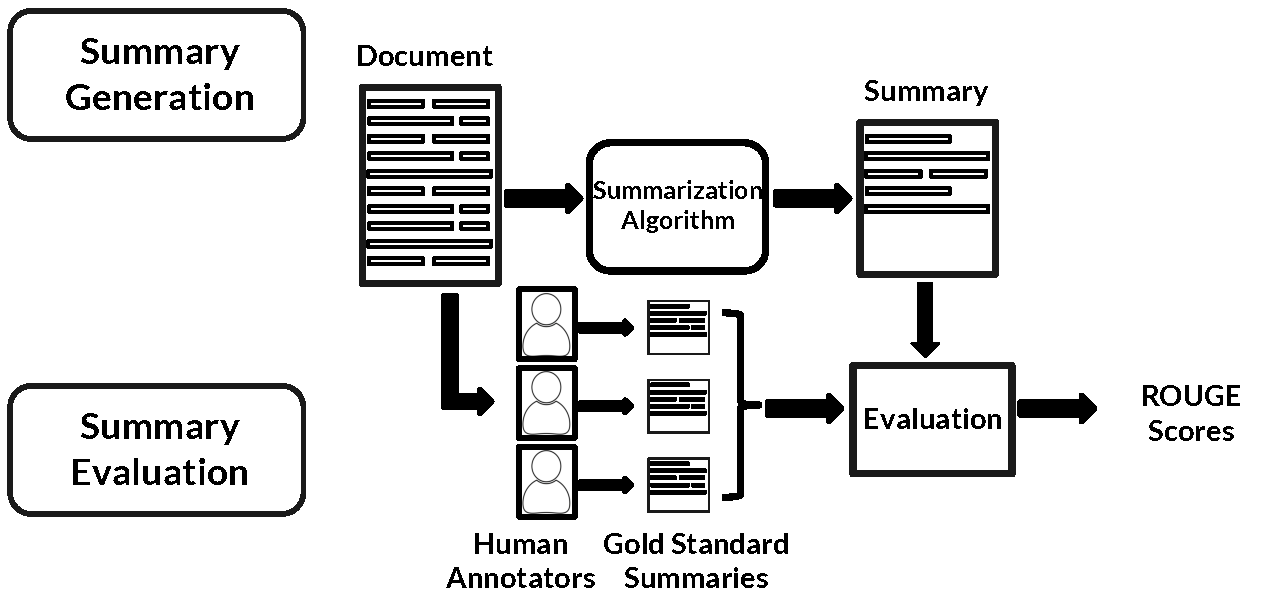
\includegraphics[width= \textwidth, height=4cm]{figures/Summarization.pdf}
		%\vspace*{-4mm}
		%\caption{}
		%\label{Fig: backpack1}
	\end{subfigure}%
	%\hfill
	%\vspace*{-4mm}
	\caption{{\bf A generic block diagram explaining text-summarization pipeline. Machine generated summaries are evaluated based on how well they match human written reference summaries. Metrics such as ROUGE scores quantify the goodness of such  automated summaries.}}
	\label{Fig: Summarization}
	\vspace{-6 mm}
\end{figure} 

Traditional summarization algorithms are meant for summarizing homogeneous documents (e.g. %one or a few 
news article(s) on a topic, or research paper(s)) and they have only focused on {\it summary-worthiness} of textual units while deciding on whether to include or exclude them in the summary. However, with the  growing popularity of social media websites, e.g. Facebook, Twitter, user-generated content constitutes a large chunk of the textual information generated on the Web today. On social media, different user groups discuss different socio-political issues, and it has been observed that they often have very different opinions on the same topic or event~\cite{dash2019summarizing,mukherjee2020read}. 
Hence, the textual information to be summarised has gradually become heterogeneous. 
In our prior work~\cite{dash2019summarizing}, we have shown that such text often contains very different opinions from people of different ideologies, social groups, etc. In many downstream applications, algorithm-generated summaries are consumed by people and hence they often play a vital role in shaping their opinion in different socio-political issues. Hence, along with summary quality, the fairness aspect of algorithmic summaries (that are produced by automatic summarization algorithms) have also become essential~\cite{shandilya2018fairness, dash2019summarizing}. Lately, this has led to different fair summarization algorithms for heterogeneous user generated textual units~\cite{dash2019summarizing, mukherjee2020read}.

\vspace{1 mm}
\noindent
\textbf{Evaluation of algorithmic summaries:} 
Traditionally, the evaluation of algorithmic summaries are carried out by evaluating how closely they match human-generated summaries.
The same source document (or set of documents) is given to a number of human annotators to summarize. Metrics like ROUGE~\cite{lin2004rouge}, ROUGE2.0~\cite{ganesan2015rouge}
are used to quantify the goodness of the algorithmic summaries. Even though these measures perform very well in evaluating the goodness of summaries (based on textual quality and readability etc.), they do not explicitly quantify the (un)fairness of an algorithmic summary. 
Moreover, this process of evaluation is often laborious and hence an expensive task. %Most existing evaluation methods require certain forms of human involvement, thus are supervised.  They either directly let humans rate the generated summaries (e.g. Pyramid [15]), elicit human-written reference summaries and measure their overlap with the generated summaries ROUGE[13], ROUGE 2.0 etc.), or collect some human annotations [8] to learn a summary evaluation function. 
Evaluation in multi-document summarization is particularly expensive. It is reported that 3,000 hours of human effort is required to evaluate the summaries from the Document Understanding Conferences (DUC)~\cite{lin2004rouge}.  

\vspace{1 mm}
\noindent
\textbf{Drawbacks in the existing framework:} 
The existing fair summarization algorithms have mostly tried to incorporate normative representational fairness goals from the perspective of the content producers/writers in the final summary. 
However, {\it whether the summaries are perceived to be fair by the consumers/readers} is still up for debate. %Moreover, none of the prior works could point out any sacrosanct definition of fairness in the context of summarization. 
Additionally, the different existing approaches of evaluating summaries (the most popular being computation of ROUGE scores) have several limitations when it comes to quantification of fairness aspect of the summaries of heterogenous user-generated text corpora. 

\vspace{1 mm}
\noindent
\textbf{Current work:} In this work, we posit that in the context of summarization, fairness is highly context-dependent, and ideally involves multiple stakeholders. 
The most important stakeholders in a summarization set up are: producers or writers of the textual units, and consumers or readers of the final summary.\footnote{We use the word-pairs `producers' and `writers', as well as `consumers' and `readers' interchangeably throughout this paper.} 
However, the interpretation of fairness may vary when we envisage it from the reader's perspective. To this end, in this work, we investigate the interplay between the earlier proposed definitions of fairness in summarization and the consumers' perceptions of fairness, and how this interplay varies with the context of the underlying topic. Further, we also investigate the effectiveness of existing measures, e.g. ROUGE in quantifying the (un)fairness of a summary. 

Specifically, we seek for the answer to the following research questions (RQs). 
RQ1:~Is the readers' perception of (un)fairness in summaries context-dependent?, 
RQ2:~Do traditional metrics for summary quality such as ROUGE scores capture readers' perception of fairness of summaries?, and finally, 
RQ3:~Can a metric based on `representation of opinions’ better capture readers’ perception of (un)fairness in summaries? 
To answer the aforementioned RQs, we conducted a series of surveys on two socio-political datasets (obtained from~\cite{dash2019summarizing}) of microblogs/tweets related to (i)~the US Presidential Elections, and (ii)~the MeToo movement. 
Through the different analyses, the main contributions/observations of the present work can be summarised as follows:
\begin{enumerate}
	\item We show that readers can differentiate between fair and unfair summaries. However, the reasons why a summary is perceived to be (un)fair is context-dependent. In some cases, the perceived fairness agrees with standard representational fairness notions for demographic groups of producers; while in other cases, the perceived fairness seems to agree more with how fairly various opinions are represented in the summary.
	\item In either case, standard ROUGE metrics cannot capture the bias in summaries as perceived by the consumers.
	\item We propose a metric for perceived bias in a summary, based on manual identification of opinions in the input text, and then judging how well various opinions are represented in the summary.
	\item Finally, we propose a graph-based methodology for automatically measuring the bias in a summary. We observe that correlates well with the perceived opinion bias metric stated above.
\end{enumerate}

%======commented out======================
\if 0
Evaluating the quality of machine-generated summaries is a highly laborious and hence an expensive task. Most existing evaluation methods require certain forms of human involvement, thus are supervised: they either directly let humans rate the generated summaries (e.g. Pyramid \cite{nenkova2004evaluating}), elicit human-written reference summaries and measure their overlap with the generated summaries  ROUGE\cite{lin2004looking}) , or collect some human annotations\cite{gao2019preference} to learn a summary evaluation function. Evaluation in multi-document summarization is particularly expensive: Lin\cite{lin2004rouge} reports that it requires 3,000 hours of human effort to evaluate the summaries from the Document Understanding Conferences (DUC). 
Various metrics have been proposed over time for quantification of the quality of summary. Some of the most popular ones are:
ROUGE metric: The metrics compare an automatically produced summary or translation against a reference or a set of references (human-produced) summary or translation. 
ROUGE 2.0 metric: It has several updated measures of ROUGE: ROUGE-N+Synonyms, ROUGE-Topic, ROUGETopic+Synonyms, ROUGE-TopicUniq and ROUGE-TopicUniq+Synonyms; all of which are improvements over the core ROUGE measures.
 There exist a few unsupervised evaluation methods (Sun and Nenkova, 2019\cite{sun2019feasibility}), but they have low correlation with human relevance ratings at summary level: given multiple summaries for the same source documents

Our main contributions in this work are:
\begin{enumerate}
 \item We show that human beings (primarily consumers who read summaries) can differentiate between fair and unfair summaries. However, the reasons why a summary is perceived to be fair / unfair  (by consumers) is context-dependent -- in some cases, the perceived fairness agrees with standard fairness notions on demographic groups of producers, while in other cases , the perceived fairness seems to agree more with how fairly various opinions are represented in the summary.
 \item In either case, standard ROUGE metrics cannot capture the bias in summaries as perceived by the consumers.
\item We propose a metric for perceived bias in a summary, based on manual identification of opinions in the input text, and then judging how well various opinions are represented in the summary.
\item We propose a graph-based methodology for automatically measuring the bias in a summary, that correlates well with the perceived opinion bias metric stated above.
\end{enumerate}
\fi 